
I am, Manohar Raavi, pursuing PhD in Engineering(Security). My major goal on taking CS6000 course is to improve my research skills. 
I am confident that the course is well designed and would make me a better researcher by the end of the semester.
 I did my Undergraduate degree in Electronics and Communications Engineering from Jawaharlal Technological University Kakinada and Masters degree in Telecommunications Management from Oklahoma State University. I worked as a Network Engineer at Oklahoma State University for almost 2 years. I like to spend most of my free time in Rec Center.
 I love to learn and play new games all the time. I play Badminton, Volleyball, Cricket, Table Tennis, Racquetball, Chess, Carrom Board etc.

\subsection{Questions and Answers}
\subsubsection {Question \#1}
Keith here. Congratulations as well on starting Ph.D. program. How did you decide on Oklahoma and UCCS to pursue your advance degrees?

Hi Keith,
Thank you. I did my Undergraduate in Electronics \& Communications Engineering and wanted to stay in communications field.
Oklahoma State University had Masters in Telecommunications program that got my attension. For Ph.D, it has to be the research and I found that UCCS faculty are doing excellent research in Security (Wireless).



\subsubsection {Question \#2}

Second question here.

\begin{figure}[htp]
    \centering
    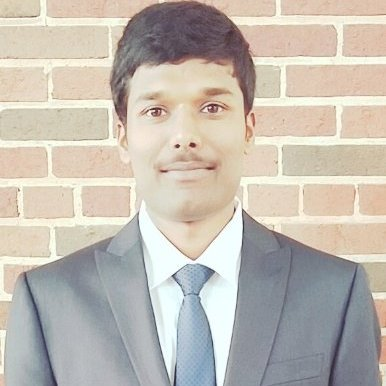
\includegraphics[width=4cm]{linkd1}
\end{figure}

Any Questions?
Hi Raavi, whats your favorite game?, Rodger